\documentclass{article}

\usepackage{url} 

\usepackage{pdfpages}
\usepackage{lastpage}
\usepackage{fancyhdr}
\usepackage{ngerman}
\usepackage{listings}

\usepackage{tabularx}
\usepackage{floatrow}
\usepackage[tableposition=top]{caption}
\floatsetup[table]{capposition=top}

\usepackage{amsmath, amssymb}

\usepackage[utf8]{inputenc}


\usepackage[numbib]{tocbibind}



\newcommand\twodigits[1]{%
   \ifnum#1<10 0#1\else #1\fi
}



\lhead{Interferometer}
\rhead{13. November 2020\\T. Maier, J. Winkler}
%\cfoot{\twodigits{\thepage}~/ \pageref{LastPage}}
\cfoot{{\thepage}~/ \pageref{LastPage}}

\newcommand{\W}{\text{W}}
\newcommand{\V}{\text{V}}
\newcommand{\A}{\text{A}}


\newcommand{\mini}{\operatorname{min}}


\begin{document}

\parindent0cm

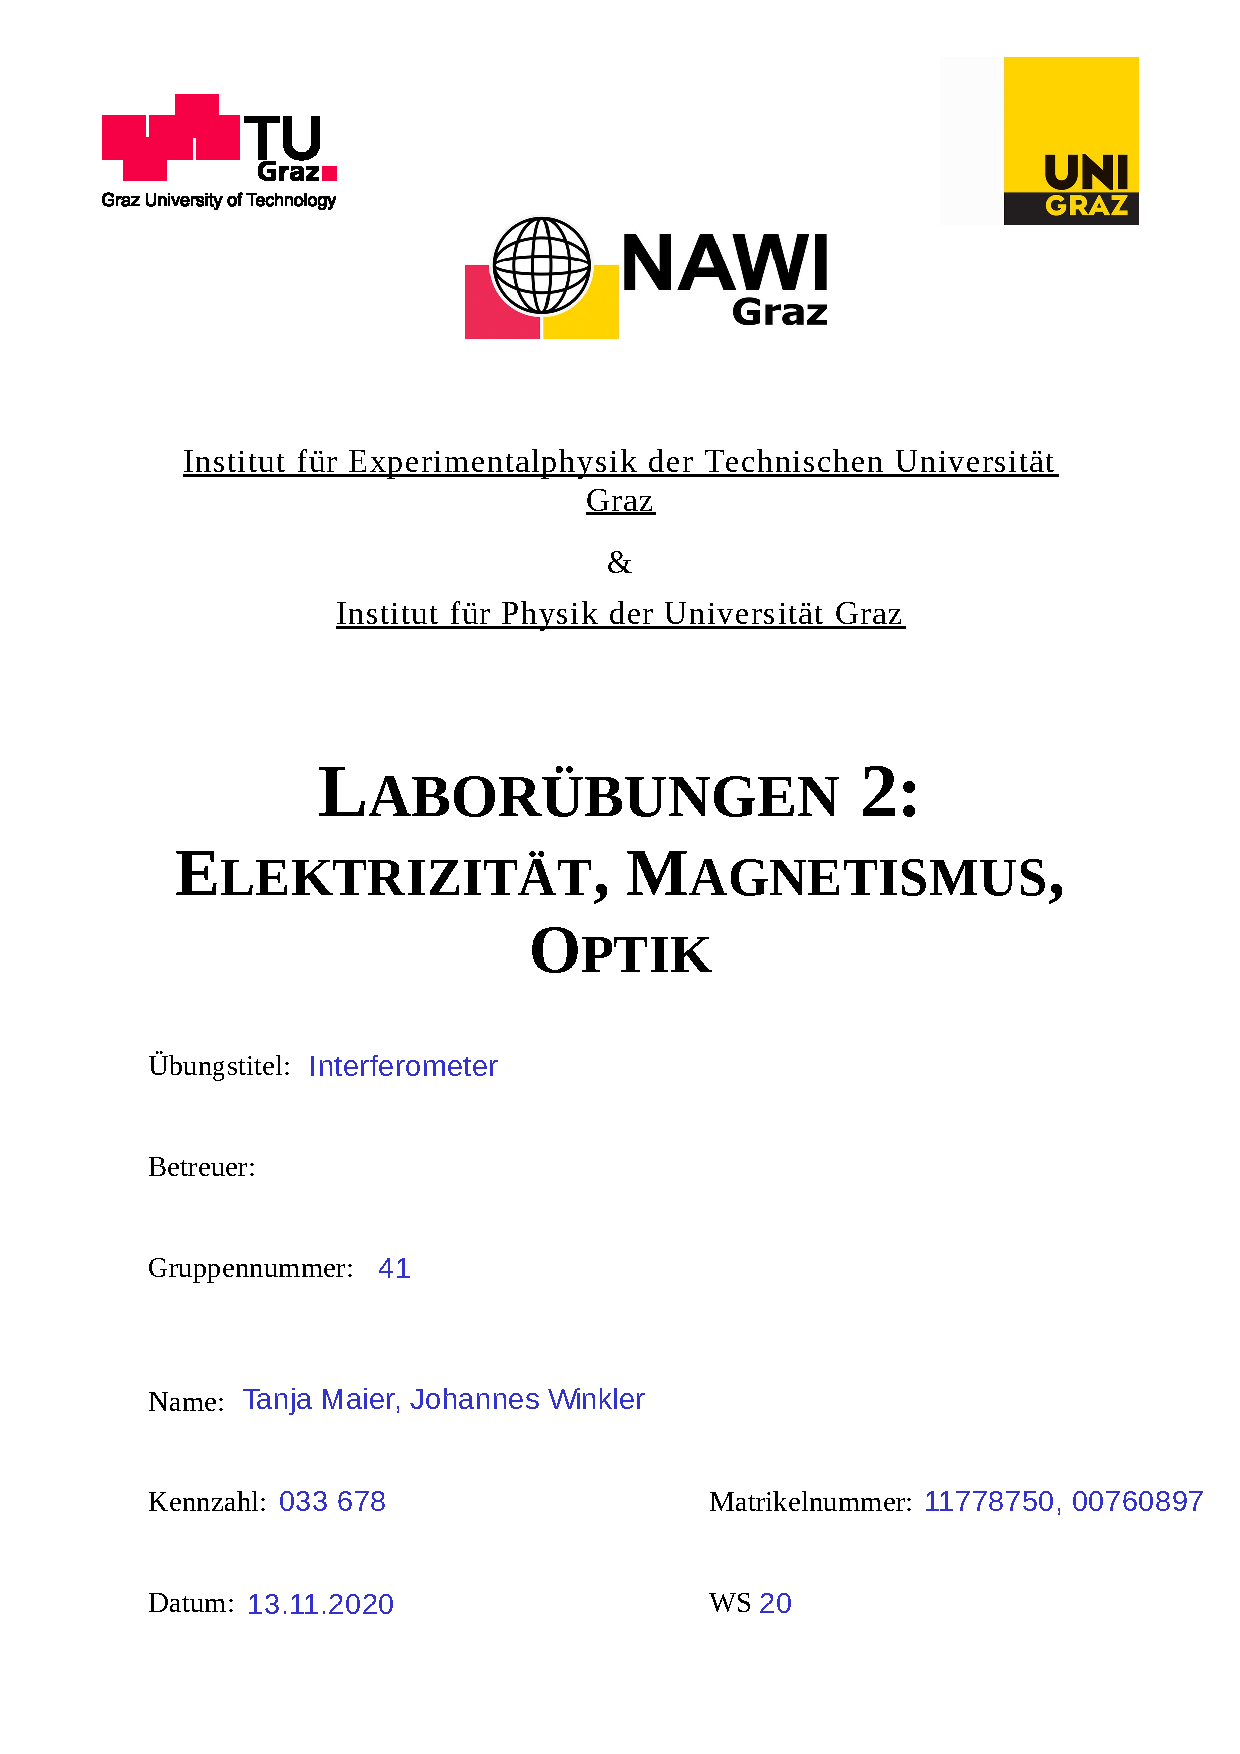
\includepdf{Deckblatt.pdf}


\pagestyle{fancy}

\tableofcontents
\newpage
\section{Aufgabenstellung}

\begin{enumerate}
\item Demonstration und Erklärung des Einflusses der Größe einer Lichtquelle auf das Interferenzmuster eines Doppelspaltes.
\item Demonstration und Erklärung des Einflusses der spektralen Breite des Lichtes einer räumlich kohärenten Lichtquelle auf das Interferenzmuster eines Doppelspaltes.
\item Bestimmung der Dicke einer Kunststoffschicht mit dem Doppelspalt Interferenzmuster.
\item Bestimmung der Größe der Lichtquelle, bei der für Doppelspalten mit unterschiedlichem Spaltabstand das Licht noch räumlich kohärent ist.
\end{enumerate}



\section{Voraussetzungen und Grundlagen}

Grundlage dieses Versuchs bietet die Wellennatur des Lichts. Licht kann als elektromagnetische Welle im sichtbaren Spektralbereich gesehen werden. Das von einer Quelle ausgesendete Licht kann dann mit einem Doppelspalt in mehrere Teilwellen aufgespalten werden. Wenn dieses Teilwellen dann wieder aufeinandertreffen (z.B. durch Totalreflexion an einem Spiegel), so kommt es je nach Gang- bzw. Zeitunterschied entweder zur Auslöschung (destruktive Interferenz) oder Verstärkung (konstruktive Interferenz) der wieder vereinigten Welle. Wichtig ist dabei, dass die Welle sowohl zeitlich als auch räumlich kohärent (Amplitude und Phase sind also an jedem Punkt und zu jeder Zeit eindeutig definiert) ist. Dann gilt
\begin{align}
\Delta s = d \cdot \sin \theta_n = n\cdot \lambda \qquad n\in \mathbb{N}_0
\end{align}
wobei der Gangunterschied der beiden Teilwellen $n$-ter Ordnung, $d$ der Abstand der Spalten, $\theta_n$ der $n$-te Beugungswinkel, n die Ordnung des Interferenzmaximums und $\lambda$ die Wellenlänge ist.

Die Interferenzmaxima werden außerdem mit einer Sammellinse erfasst und abgebildet. Für den Abstand $b_n$ zwischen $0$-tem und $n$-tem Maximum gilt folgender Zusammenhang 
\begin{align}
b_n = f_2 \cdot \tan\left( \operatorname{arcsin}\left(\frac{n\cdot\lambda}{d}\right)\right), \qquad n\in\mathbb{N}_0
\end{align}
wobei $f_2$ die Brennweite der Sammellinse nach dem Doppelspalt ist. Außerdem kann man noch den Kontrast $K$ des Inferenzmusters bestimmen, welcher von der jeweiligen Intensität der Lichtquelle abhängt.
\begin{align}
K = \frac{I_\text{0,max}-I_\text{1,min}}{I_\text{0,max}+I_\text{1,min}} \label{eq:kontrast}
\end{align}
wobei $I$ die Intensität, $f_1$ die Brennweite der Sammellinse vor dem Doppelspalt und $\omega$ der Radius der Lichtquelle ist. Außerdem wird bei diesem Experiment auch eine Probe mit Polyacrylat verwendet, welche eine zusätzliche Phasenverschiebung am Doppelspalt bewirkt. Diese Phasenverschiebung kann beschrieben werden durch
\begin{align}
\Delta s_0 = \Delta s + t\cdot (n_1-n_2) = d\cdot\sin(\theta)\cdot t\cdot (n_1-n_2)
\end{align}
wobei $t$ die Dicke der Probe, $n_1$ der Brechungsindex der Probe und $n_2$ der Brechungsindex der Umgebung (hier: Luft, also n2 = 1) ist.


%\begin{figure}[H]
%\caption{Transformator}
%\label{fig:transformator}
%{\centering
%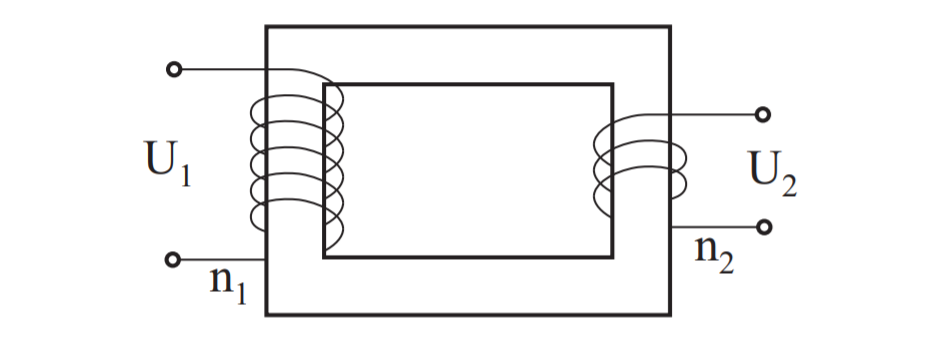
\includegraphics[scale=0.4]{transformator.png}
%~
%}
%\end{figure}





\section{Geräteliste}

\begin{table}[H]
\caption{Liste der verwendeten Geräte}

~

\begin{tabular}{l|p{3cm}p{3cm}llll}
Abk. & Bezeichnung  & Typ & Gerätenummer & Unsicherheit \\
\hline
S & Spaltblende \\
\hline
L1 & Sammellinse 1 & $f_1 = 300~$mm & & $\Delta f_1 = 0.5~$mm \\
\hline
L2 & Sammellinse 2 & $f_2 = 150~$mm & & $\Delta f_2 = 0.5~$mm \\
\hline
L3 & Sammellinse 3 & $f_3 = 40~$mm & & $\Delta f_3 = 0.5~$mm \\
\hline
L4 & Sammellinse 4 & $f_4 = 30~$mm & & $\Delta f_4 = 0.5~$mm \\
\hline
DS & Doppelspalt \\
\hline





B & Lochblenden und Irisblende & $d_1=2~$mm ~ ~ ~ ~ $d_2=3~$mm   ~~~~~~~~~~~~ $d_3=6~$mm & &  $\Delta d = 0.1~$mm \\
\hline
F & Filterrad für LEDs & \\
\hline
K & Kamera
\end{tabular}

\end{table}



\section{Beschreibung der Versuchsanordnung}

Der Versuchsaufbau ist maßstabsgetreu in Grafik \ref{fig:aufbau} dargestellt.
\begin{figure}[H]
\caption{Versuchsaufbau. $L_1,L_2,L_3,L_4$ Linsen, $S$ Spaltblende, $DS$ Doppelspalt, $F$ Filterrad, $O$ Substrat mit Polyacrylat-Schicht, $K$ Kamera. Maßstab 1:20}
\label{fig:aufbau}
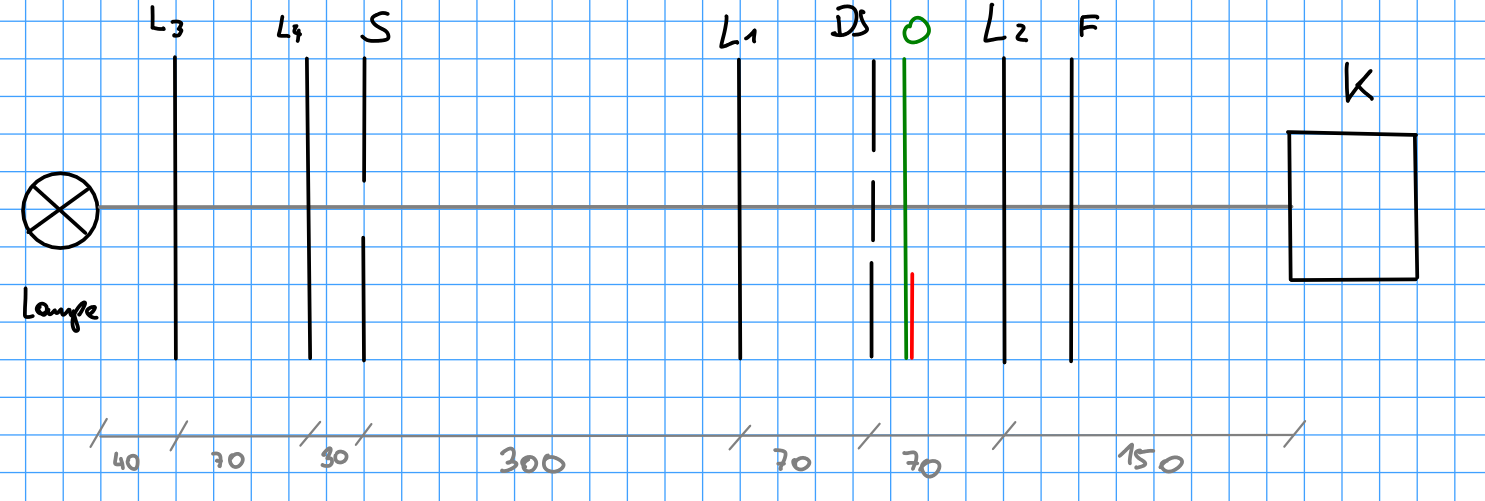
\includegraphics[scale=1]{aufbau.png}
\end{figure}


Die von der Lampe ausgehenden Lichtstrahlen werden in $L_3$ parallelisiert, da der Abstand zur Lampe genau die Brennweite von $L_3$ ist. In $L_4$ wird der Strahl auf den Spalt fokussiert. Die einstellbare Spaltblende liegt exakt im Brennpunkt von $L_1$ und $L_4$, daher werden die ausgehenden Strahlen in $L_1$ wieder parallelisiert. Danach trifft das Licht auf den Doppelspalt, wo Beugung stattfindet. Danach dringt das Licht durch das Substrat, dass teilweise mit einer Schicht Polyacrylat versehen ist. Das Beugungsmuster wird von $L_2$ auf eine Kamera umgeleitet, die sich genau im Brennpunkt von $L_2$ befindet. Zwischen $L_2$ und der Kamera ist zusätzlich noch ein Filterrad, welches wo man wahlweise einen Bandpass (633~nm) oder einen Langpass dazwischen schalten kann. Grafik \ref{fig:strahlen} zeigt den Strahlengang im Interferometer. 

\begin{figure}[H]
\caption{Strahlengang im Interferometer. Die Strahlen sind in blau eingezeichnet, die 1. Beugungsordnung in orange. Maßstab 1:20}
\label{fig:strahlen}
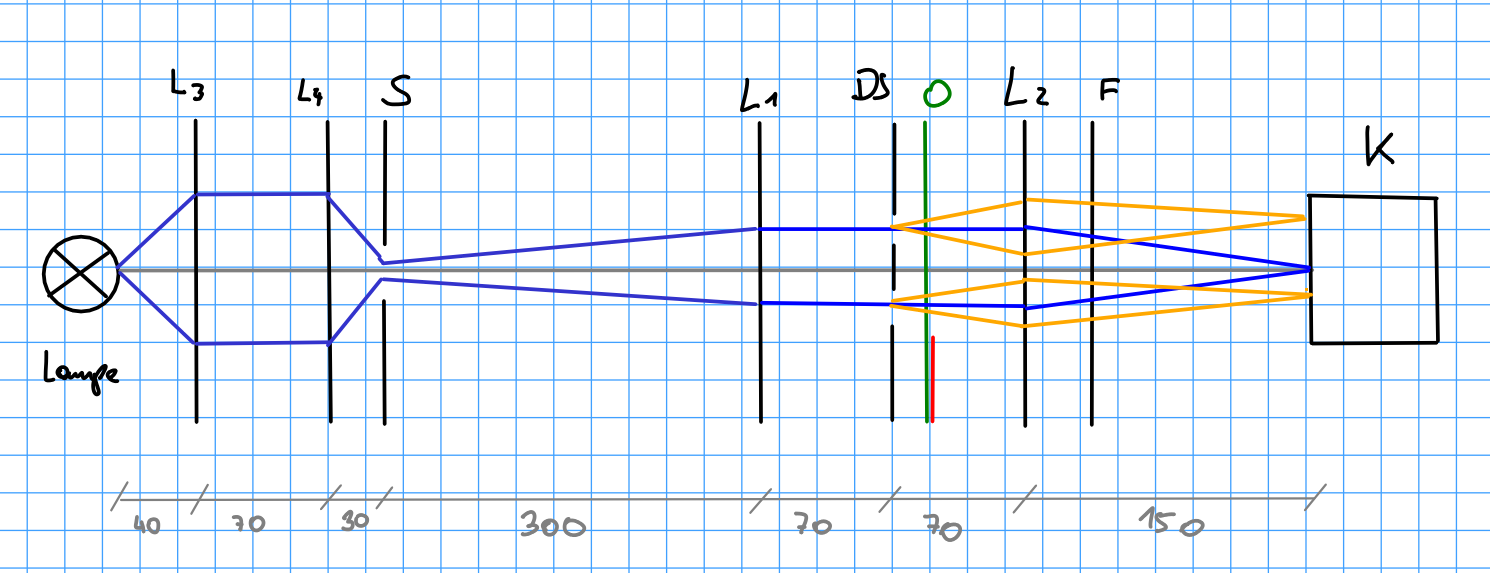
\includegraphics[scale=1]{strahlen.png}
\end{figure}



\section{Versuchsdurchführung und Messwerte}

Die Versuchsergebnisse werden von der Kamera aufgenommen. Diese wird mit einem Computer und der Software \textit{IC Capture} gesteuert.


\subsection{Teil 1: Zusammenhang zwischen Größe der Lichtquelle und Interferenzmuster}

Bei einer großen Lichtquelle kann räumliche Kohärenz auftreten. Daraus resultiert ein schwächerer Konstrast. Die Größe der Lichtquelle wird durch die verstellbare Spaltblende realisiert. Für diesen Versuch wurde monochromatisches Licht verwendet. Dann wurde der $633~$nm Bandpassfilter in den Strahlengang gedreht und der mittlere Doppelspalt in den Strahlengang geschoben.

Dann wurden 6 geeignete Größen der Lichtquelle gewählt, um den Verlauf des Kontrastes gemäß im Bereich $0 < 2\cdot w < 1.5 \cdot \lambda\cdot f_1 / d$ darstellen zu können. Dafür wurde zunächst die Spaltbreite des Kontrast-Minimums bestimmt. Beim Wert 0 der Mikrometerschraube war der Spalt jedoch noch nicht ganz geschlossen, sodass mit einer negativen Spaltbreite begonnen wurde, um den Spalt auch ganz geschlossen zu halten.
Für die gewählten Größen der Lichtquelle wurde jeweils ein Foto des Beugungsmusters aufgenommen und zusätzlich werden die Grauwerte mit dem Programm ImageJ grafisch dargestellt.

Der Konstrast kann nun mit Formel~\ref{eq:kontrast} berechnet werden.

Die Aufnahmen der Interferenzmuster und die grafische Darstellung der Grauwerte sind im folgenden aufgelistet.

\begin{figure}[H]
\centering
\caption{...}
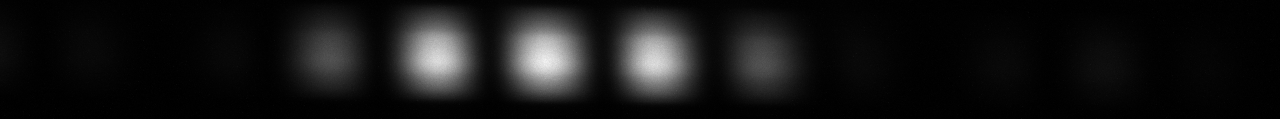
\includegraphics[width=9cm]{moodle/img2.png}
\end{figure}

\begin{figure}[H]
\centering
\caption{...}
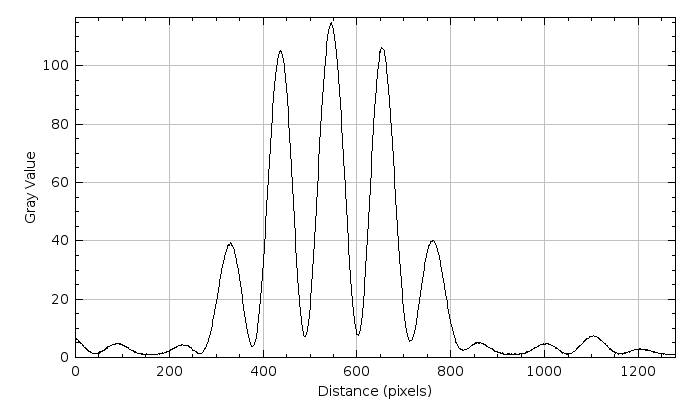
\includegraphics[width=9cm]{moodle/img2_graph.png}
\end{figure}



\begin{figure}[H]
\centering
\caption{...}
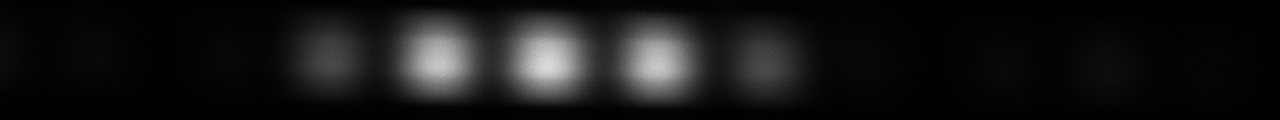
\includegraphics[width=9cm]{moodle/img3.png}
\end{figure}

\begin{figure}[H]
\centering
\caption{...}
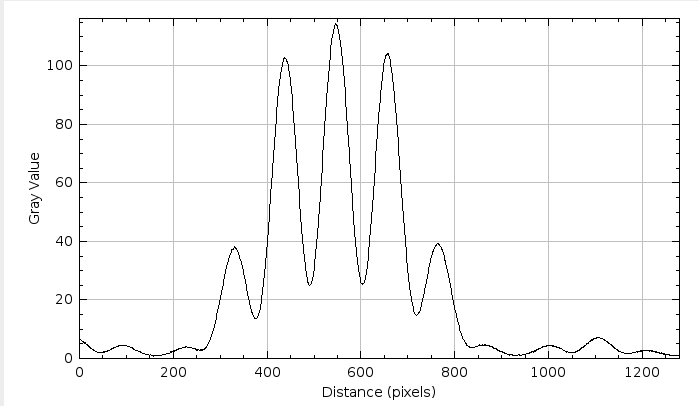
\includegraphics[width=9cm]{moodle/img3_graph.png}
\end{figure}



\begin{figure}[H]
\centering
\caption{...}
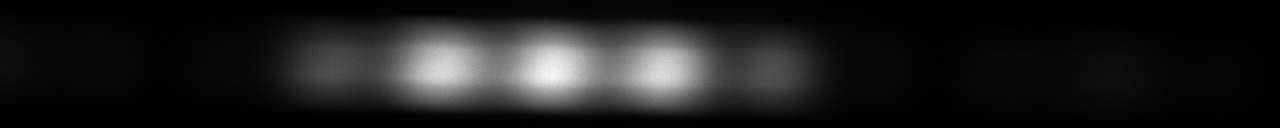
\includegraphics[width=9cm]{moodle/img4.png}
\end{figure}

\begin{figure}[H]
\centering
\caption{...}
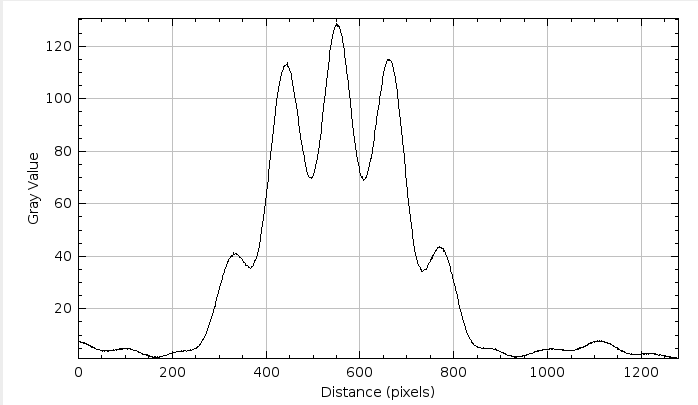
\includegraphics[width=9cm]{moodle/img4_graph.png}
\end{figure}




\begin{figure}[H]
\centering
\caption{...}
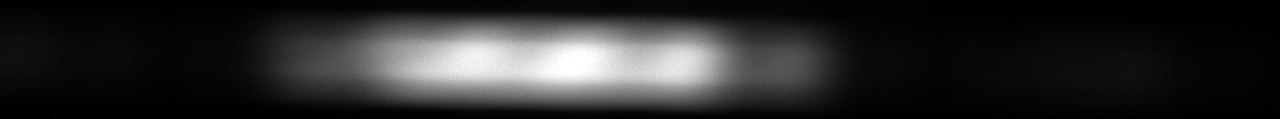
\includegraphics[width=9cm]{moodle/img5.png}
\end{figure}

\begin{figure}[H]
\centering
\caption{...}
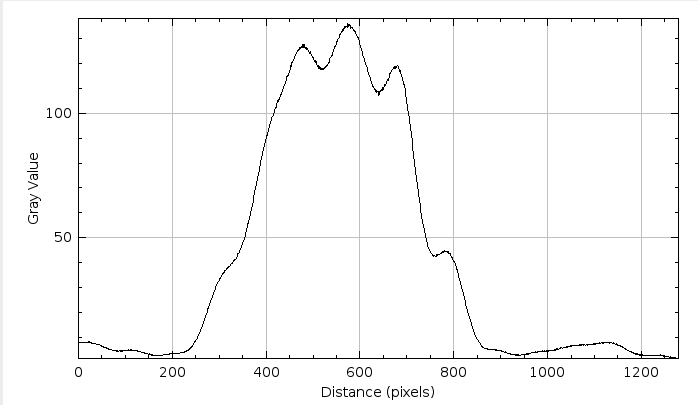
\includegraphics[width=9cm]{moodle/img5_graph.png}
\end{figure}



\begin{figure}[H]
\centering
\caption{...}
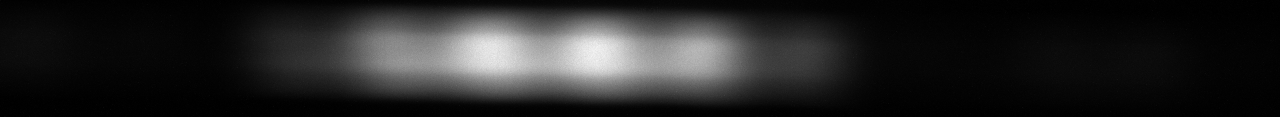
\includegraphics[width=9cm]{moodle/img6.png}
\end{figure}

\begin{figure}[H]
\centering
\caption{...}
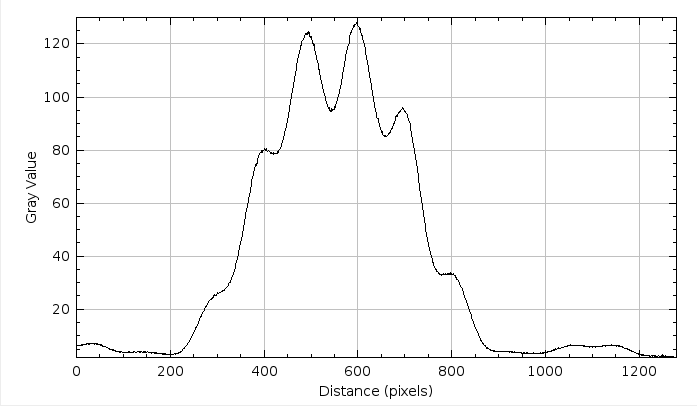
\includegraphics[width=9cm]{moodle/img6_graph.png}
\end{figure}





\begin{figure}[H]
\centering
\caption{...}
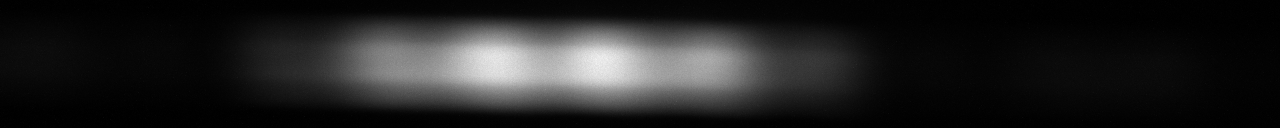
\includegraphics[width=9cm]{moodle/img7.png}
\end{figure}

\begin{figure}[H]
\centering
\caption{...}
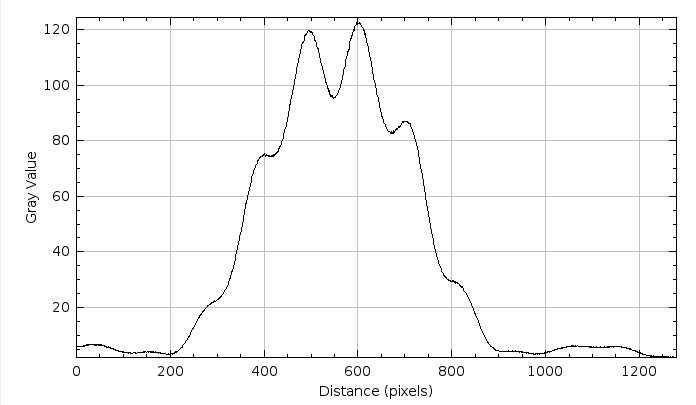
\includegraphics[width=9cm]{moodle/img7_graph.png}
\end{figure}



\begin{table}[H]
\caption{Beugungsextremum 0. Ordnung, bezeichnet als $I_0$, Beugungsextrema 1. Ordnung $I_{-1}$ links von $I_0$ und $I_{+1}$ rechts von $I_0$. Die 0. Ordnung ist bei den ersten Messungen ein Maximum, wird aber später zu Minimum wegen Nullstelle im Kontrast.}
\begin{tabular}{l|rrrr}
Spaltbreite & $I_0$ & $I_{-1}$ & $I_{+1}$ & $\overline{I_{1}}$ \\
\hline
 & 114.891 & 7.118 & 7.597 & 7.358 \\
 & 114.552 & 24.817 & 25.261 & 25.039 \\
 & 128.655 & 69.862 & 69.026 & 69.444 \\
 & 135.926 & 117.512 & 107.198 & 112.355 \\
 & 94.551 & 124.517 & 128.076 & 126.297 \\
 & 95.355 &  119.835 & 122.570 & 121.202
\end{tabular}
\end{table}





%
%\begin{table}[H]
%\caption{Beugungsextremum 0. Ordnung, bezeichnet als $I_0$, Beugungsextrema 1. Ordnung $I_{-1}$ links von $I_0$ und $I_{+1}$ rechts von $I_0$. Die 0. Ordnung ist bei den ersten Messungen ein Maximum, wird aber später zu Minimum wegen Nullstelle im Kontrast.}
%\begin{tabular}{l|rrrr}
%Spaltbreite & $I_0$ & $I_{-1}$ & $I_{+1}$ & $\overline{I_{1}}$ \\
%\hline
% & 114.891 & 7.118 & 7.597 & 7.358 \\
% & 114.552 & 24.817 & 25.261 & 25.039 \\
% & 128.655 & 69.862 & 69.026 & 69.444 \\
% & 135.926 & 117.512 & 107.198 & 112.355 \\
% & 94.551 & 124.517 & 128.076 & 126.297 \\
% & 95.355 &  119.835 & 122.570 & 121.202
%\end{tabular}
%\end{table}


\newpage
\subsection{Teil 2: Zusammenhang zwischen spektraler Breite und Interferenzmuster}

Beim zweiten Versuch ist diesmal das Licht räumlich kohärent, dafür variiert die spektrale Breite (und damit die zeitliche Kohärenz). Die Theorie sagt, dass die 0. Beugungsordnung mit der höchsten Intensität dargestellt wird und die Intensität nach außen hin nachlässt. Es wurde die Spaltblende so eingestellt, dass das Licht mit 0.43 mm Spaltabstand räumlich gut kohärent ist. Danach wurde ein Beugungsbild mit dem 633 nm Bandpassfilter, mit dem Langpassfilter und ohne Filter aufgenommen. 

\begin{figure}[H]
\centering
\caption{Beugungsmuster mit Langpassfilter}
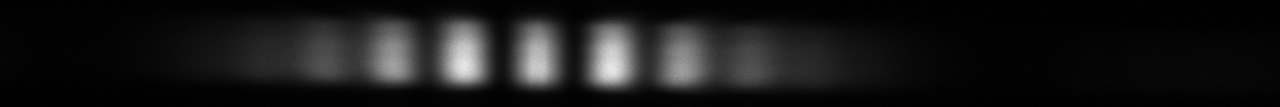
\includegraphics[width=9cm]{moodle/img_LP.png}
\end{figure}

\begin{figure}[H]
\centering
\caption{Beugungsmuster mit 633~nm-Bandpassfilter}
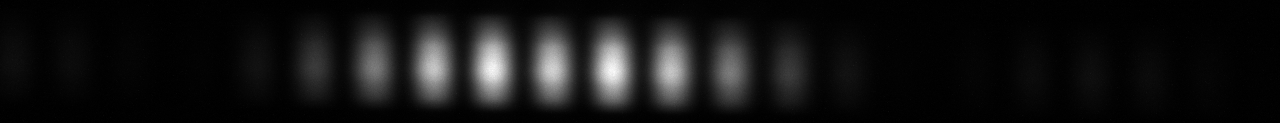
\includegraphics[width=9cm]{moodle/img_633BP.png}
\end{figure}

\begin{figure}[H]
\centering
\caption{Beugungsmuster ohne Filter}
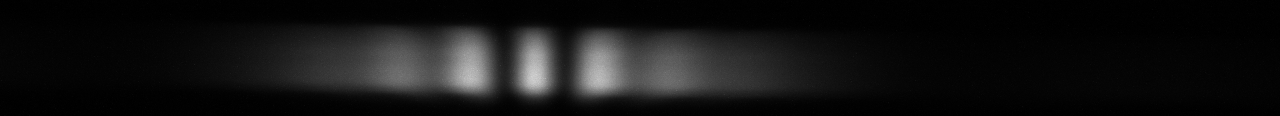
\includegraphics[width=9cm]{moodle/img__.png}
\end{figure}

\begin{figure}[H]
\centering
\caption{Transmissionsspektrum des Langpassfilters (blau) und des Bandpassfilters (orange). Quelle: \cite{quelle6}}
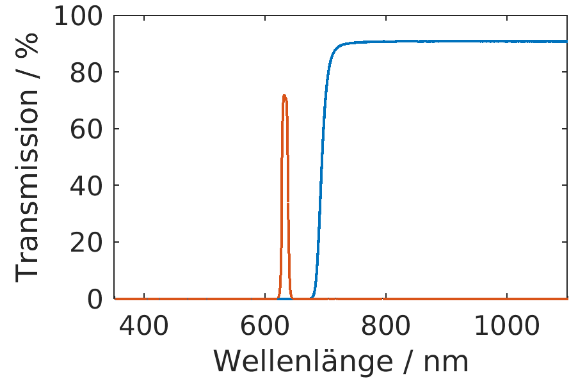
\includegraphics[width=5cm]{moodle/filter.png}
\end{figure}



\subsection{Teil 3: Bestimmung der Dicke der Polyacrylat-Schicht anhand des Interferenzmusters}

Hier wurde der vorderste Doppelspalt mit 0.43 mm Spaltabstand verwendet und alle Filter aus dem Strahlengang gedreht. Danach wurde die mit Polyacrylat überzogene Probe in den Strahlengang eingebracht und mit einer Justierschraube verschoben, sodass die Polyacrylat-Schicht nur einen der beiden Spalte abdeckt. Dann wurde das Bild des verschobenen und ein Bild des nicht verschobenen Beugungsmusters, sowie ein Bild ohne Polyacrylat als Referenzwert aufgenommen.

\begin{figure}[H]
\centering
\caption{Darstellung des Beugungsmusters mit und ohne Verschiebung}
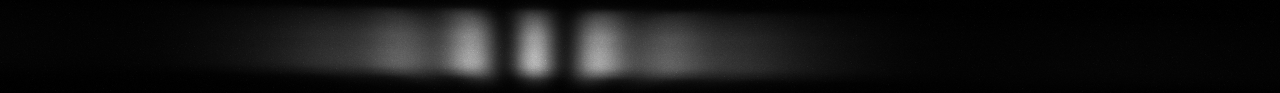
\includegraphics[width=9cm]{moodle/img_noShift.png}
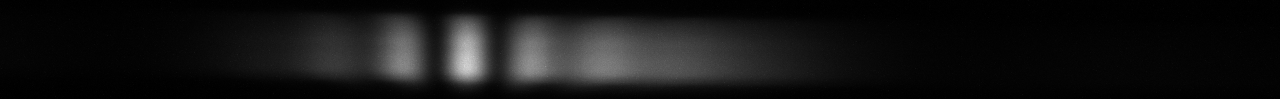
\includegraphics[width=9cm]{moodle/img_Shift.png}
\end{figure}


\subsection{Teil 4: Maximale Größe des Lichts für räumliche Kohärenz}

In diesem Versuch wurde wieder monochromatisches Licht mit einem Bandpass von 633 nm verwendet. Für drei Doppelspalten ($d_1=0.43~$mm, $d_2=0.23$~mm und $d_3=0.13$~mm) wird die Blende so reguliert, dass der Kontrast gerade verschwindet. Die Werte werden an der $\mu$m-Schraube abgelesen.

\begin{table}[H]
\caption{Ablesewerte der Mikrometerschraube. $x_1$ sind die Werte für den Spalte mit $d_1=0.43$~mm, $x_2$ für den Spalte mit $d_2=0.23$~mm und $x_3$ für den Spalt mit $d_3=0.13~$mm. Berechnung des Mittelwertes und der Standardabweichung.}
\begin{tabular}{c|rrr}
Messung & $x_1$ / mm & $x_2$ / mm & $x_3$ / mm \\
\hline
1 & 0.325 & 0.695 & 1.740 \\
2 & 0.315 & 0.722 & 1.865 \\
3 & 0.322 & 0.715 & 1.900 \\
4 & 0.318 & 0.725 & 1.655 \\
\hline 
$\overline{x_i}$ & 0.320 & 0.714 & 1.790 \\
$\sigma_i$ & 0.004 & 0.014 & 0.113
\end{tabular}

\end{table}



\section{Auswertung}



\subsection{Teil 1: Zusammenhang zwischen Größe der Lichtquelle und Interferenzmuster}

Gleichung~\eqref{eq:kontrast} berechnet den Kontrast. Zusätzlich betrachten wir den Betrag des Kontrasts, da wir in der Messreihe eine Nullstelle des Kontrasts haben. Mit Fehlerrechnung ergibt sich
\begin{align*}
K = \left|\frac{I_\text{0,max}-I_\text{1,min}}{I_\text{0,max}+I_\text{1,min}} \right| \pm \left| \frac{ 2\cdot I_{1,\text{min}} \cdot \Delta I_{0,\text{max}} }{(I_\text{0,max}+I_\text{1,\text{min}})^2}  + \frac{ 2\cdot I_{0,\text{max}} \cdot \Delta I_{1,\text{min}} }{(I_\text{0,max}+I_\text{1,min})^2} \right|
\end{align*}



\begin{table}[H]
\caption{Berechnung des Kontrasts, Beugungsextremum 0. Ordnung $I_0$, mittleres Beugungsextremum 1. Ordnung $I_1$.}
\begin{tabular}{l|rr|r}
Spaltbreite & $I_0$ & $I_1$ & $K$ \\
\hline
 & 114.891 &   7.358 & $0.880$ \\
 & 114.552 &  25.039 & $0.641$ \\
 & 128.655 &  69.444 & $0.299$ \\
 & 135.926 & 112.355 & $0.095$ \\
 & 94.551  & 126.297 & $0.144$ \\
 & 95.355 &  121.202 & $0.119$
\end{tabular}
\end{table}



\subsection{Teil 2: Zusammenhang zwischen spektraler Breite und Interferenzmuster}


\begin{figure}[H]
\centering
\caption{Darstellung der Intensitäten der Beugungsmaxima abhängig vom Filter.}
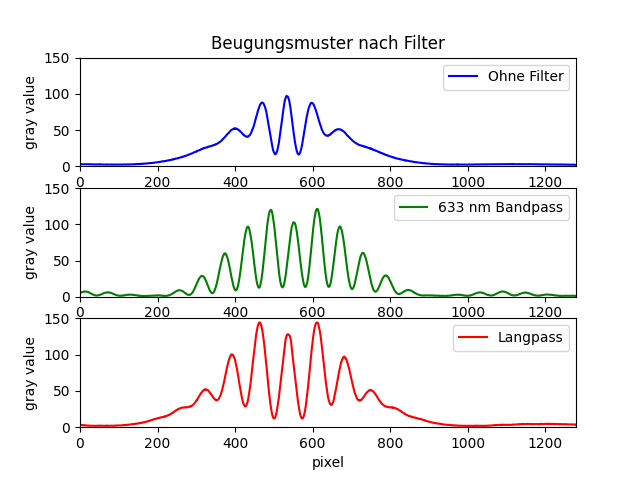
\includegraphics[width=12cm]{filter.png}
\end{figure}



\subsection{Teil 3: Bestimmung der Dicke der Polyacrylat-Schicht anhand des Interferenzmusters}

Es werden die beiden 0. Ordnungen verglichen. Ohne Polyacrylatschicht ist das gesuchte Maximum bei Pixel 534, während es ohne Polyacrylatschicht bei 467 ist. Als Unsicherheit werden 2 Pixel angenommen, da die unmittelbar benachbarten Grauwerte relativ ähnlich sind. Als Verschiebung ergibt sich
\begin{align*}
\delta = (67 \pm 4)~\text{pixel}
\end{align*}

\begin{figure}[H]
\centering
\caption{Darstellung des Beugungsmusters mit und ohne Verschiebung}
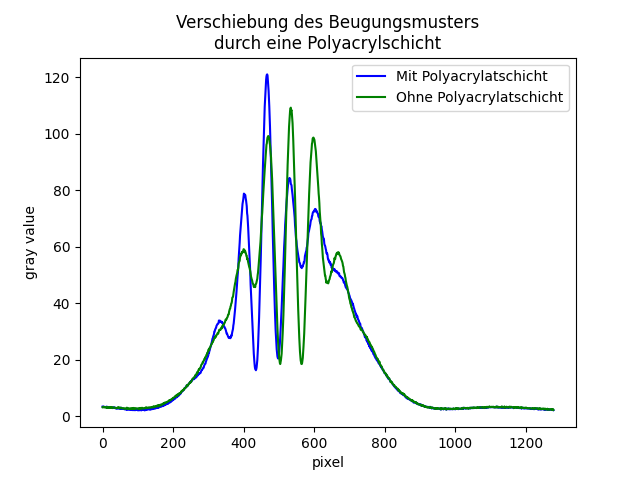
\includegraphics[width=9cm]{shift_noshift.png}
\end{figure}

\subsection{Teil 4: Maximale Größe des Lichts für räumliche Kohärenz}



\section{Diskussion}

\subsection{Teil 1: Zusammenhang zwischen Größe der Lichtquelle und Interferenzmuster}


Man sieht deutlich, dass der Kontrast zuerst mit Größe des Spaltes abnimmt. Nach einem Minimum steigt der Kontrast wieder.




\section{Zusammenfassung}




%\newpage 
%\appendix
%\section{Python Skript}



\definecolor{commentgreen}{RGB}{2,112,10}
\definecolor{eminence}{RGB}{108,48,130}
\definecolor{weborange}{RGB}{255,165,0}
\definecolor{frenchplum}{RGB}{129,20,83}

\lstdefinelanguage{python}{
    morekeywords={def, for, range, abs, return},
    otherkeywords={<-,->, |>, \%\{, \}, \{, \, (, )},
    sensitive=true,
    morecomment=[l]{\#},
    morecomment=[n]{/*}{*/},
    morecomment=[s][\color{purple}]{:}{\ },
    morestring=[s][\color{orange}]"",
    commentstyle=\color{commentgreen},
    keywordstyle=\color{eminence},
    stringstyle=\color{red},
	basicstyle=\ttfamily,
	breaklines,
	showstringspaces=false,
	frame=tb
}
%\lstinputlisting[language=Python,captionpos=b, label=lst:test,caption={Python Skript}]{generate_numbers.py}

%\lstinputlisting[language=Python,captionpos=b, label=lst:test,caption={Bessel Auswertung}]{generate_numbers_bessel.py}


%\lstinputlisting[language=Python,captionpos=b, label=lst:test,caption={Zerstreuungslinse Auswertung}]{generate_numbers_zerstreuungslinse.py}


\begin{thebibliography}{9}
\bibitem{quelle1} \url{https://www.youtube.com/watch?v=oFJCEGcwUiQ}, 07.11.2020, 00:15 Uhr
\bibitem{quelle2} \url{https://www.spektrum.de/lexikon/physik/abbesche-theorie/13}, 07.11.2020, 00:17 Uhr
\bibitem{quelle3} \url{https://www.univie.ac.at/mikroskopie/1_grundlagen/optik/opt_instrumente/7_abbe.htm}, 07.11.2020, 00:24 Uhr
\bibitem{quelle4} \url{https://physik.cosmos-indirekt.de/Physik-Schule/Rayleigh-Kriterium}, 07.11.2020, 00:26 Uhr
\bibitem{quelle5} \url{https://www.youtube.com/watch?v=PZaUY45ce8k}, 07.11.2020, 00:27 Uhr
\bibitem{quelle6} Unterlagen aus Moodle, H. Ditlbacher, bereitgestellt von der KF Universität Graz
\end{thebibliography}


\end{document}
